\documentclass[a4paper, 12pt]{extarticle}

% Import packages
%------------------------------------------------
\usepackage[utf8]{inputenc}  % utf8 encoding
\usepackage{csquotes}        % for Russian quotes
\usepackage[russian]{babel}  % enable Russian language
\usepackage{titling}         % for \thetitle, \thedate
\usepackage{enumitem}        % for list customization
\usepackage{graphicx}        % for adding images
\usepackage{prettyref}       % for configuring references
\usepackage{caption}
\usepackage{wrapfig}
\usepackage{enumitem}        % for lists customization
\usepackage{graphicx}        % for adding images
\usepackage{prettyref}       % for configuring references
\usepackage{caption}         % for figure caption customization
\usepackage{subcaption}      % for \subfigure
\usepackage{wrapfig}         % for figures and images

\usepackage{tikz}            % for diagrams
\usetikzlibrary{arrows,shapes,positioning,shadows,trees}
\tikzstyle{every node}=[draw=black,thin,anchor=west, minimum height=2.5em]

%------------------------------------------------
% Geometry
%------------------------------------------------
\usepackage{geometry}
\geometry{
    top=1.5cm,        % Top margin
    bottom=1.5cm,     % Bottom margin
    left=2cm,         % Left margin
    right=2cm,        % Right margin
    includefoot,      % Include space for a footer
}

%------------------------------------------------
% Table of Context
%------------------------------------------------
\usepackage[titles]{tocloft}                      % style of table of context
\usepackage{hyperref}                             % clickable table of context items
\setcounter{tocdepth}{2}                          % set ToC depth. (2: sections+subsubsections)
\renewcommand{\cftsecafterpnum}{\vspace{10pt}}    % set space after section
\renewcommand{\cftsubsecafterpnum}{\vspace{5pt}}  % set space after subsection
\renewcommand{\cftsecfont}{\bfseries \large}      % change section font

\hypersetup{
    colorlinks,
    citecolor=black,
    filecolor=black,
    linkcolor=black,
    urlcolor=black
}

%------------------------------------------------
% Sections style
%------------------------------------------------
\usepackage{titlesec} % for changing style of sections

% Section settings
\titleformat{\section}
{\bfseries\LARGE}
{\thesection. }
{4pt}
{}
[{\titlerule[0.4pt]}]

% Subsection settings
\titleformat{\subsection}
{\bfseries\Large}
{\thesubsection. }
{0pt}
{}

% Subsubsection settings
\titleformat{\subsubsection}
{\bfseries\large}
{}
{0pt}
{}

%------------------------------------------------
% Other settings
%------------------------------------------------
\setlength{\parindent}{0pt}
\setlist{itemsep=1pt}
\newrefformat{fig}{(рис. \ref{#1})}
\addto{\captionsrussian}{
  \renewcommand{\refname}{Список использованных источников}
}

%------------------------------------------------
% Diagrams settings
%------------------------------------------------
%------------------------------------------------
% Title, author, date
%------------------------------------------------
\title{Помощь старшеклассникам в эффективной подготовке к сдаче ЕГЭ.}
\author{Меркулов Вадим}
\selectlanguage{russian}
\date{\today}
%------------------------------------------------

\begin{document}
\begin{titlepage}
    \vspace*{0.7cm}
    \begin{center}
        \begin{figure}[h]
            
\includegraphics{../img/title_page_school_logo.jpg}
        \end{figure}
        \vspace{1.5cm}

        \Large{\textbf{
            Индивидуальный проект \\
            \textquote{\thetitle}}
        }
    \end{center}
    \vspace{5cm}

    \begin{flushright}
        Работу выполнил:\\ \vspace{7pt}
        Ученик 10 \textquote{А} класса\\ \vspace{7pt}
        \theauthor\\ \vspace{1cm}
        Научный руководитель:\\ \vspace{7pt}
    \end{flushright}
    \vfill
    \centering
    Москва, {\the\year} г.

\end{titlepage}

\tableofcontents
\newpage

\section{Введение}

\vspace{2mm}
\textbf{Актульность}
\vspace{2mm}
\\
Ни для кого не секрет, что сдача Единого Государственного Экзамена вместе с
подготовкой к ней становится значимым периодом в жизни для большей части
учеников старшей школы, заинтересованных в своем будущем. В связи с этим у
многих подростков невольно возникает вопрос, как именно стоит готовиться к
столь важному испытанию, чтобы затраченные силы были прямо пропорциональны
полученным результатам, а время подготовки впоследствии не стало предметом
сожаления?  В век переизбытка цифровой информации становится все труднее
абстрагироваться от ненужного и сфокусировать все свои усилия на одном
предмете, не распыляясь на множество задач. На мой взгляд именно сейчас
необходимо и по-настоящему актуально создать ресурс, который сможет
предоставить ученику широкий спектр заданий для выполнения, будет простым и
понятным в использовании и содержащий только необходимые материалы, напрямую относящиеся к подготовке к ЕГЭ.
\\

\vspace{2mm}
\textbf{Цель}
\vspace{2mm}
\\
Облегчение процесса подготовки к сдаче ЕГЭ путем непосредственной разработки собственного сайта.
\\

\vspace{2mm}
\textbf{Объект}
\vspace{2mm}
\\
Сниженная эффективность учащихся при самостоятельной подготовке к ЕГЭ.
\\

\vspace{2mm}
\textbf{Предмет}
\vspace{2mm}
\\
Способ повышения эффективности обучения учеников в интернете
путем разработки собственного ресурса по подготовке к экзамену.
\\

\vspace{2mm}
\textbf{Гипотеза}
\vspace{2mm}
\\
Созданный сайт сможет облегчить процесс тренировки и подготовки
старшеклассников к сдаче ЕГЭ.
\\

\vspace{2mm}
\textbf{Задачи:}
\begin{itemize}
    \item[\bfseries--] Создать интуитивно понятный сайт по подготовке к ЕГЭ
    \item[\bfseries--] Исключить ненужные данные, которые могут отвлечь
        учащегося от выполнения заданий
    \item[\bfseries--] Сделать ресурс воспроизводимым как с компьютеров, так и
        с мобильных устройств
    \item[\bfseries--] Сделать ресурс абсолютно бесплатным.
\end{itemize}

\vspace{2mm}
\textbf{Методы:}
\begin{itemize}
    \item[\bfseries--] Анализ информационных порталов с похожей специализацией
    \item[\bfseries--] Анализ потенциальных причин отвлечения внимания во время
        самоподготовки
    \item[\bfseries--] Опора на собственный опыт в подготовке к экзаменам, а
        также на опыт сверстников
\end{itemize}
\newpage

\section{Основные сведения о подготовке к Единому Государственному Экзамену}
\subsection{Современные методы самоподготовки к экзамену}
\vspace{2mm}
Современному школьнику не составляет никакого труда найти информацию по
интересующей его теме с помощью Интернета. Открытые ресурсы в разы облегчают
поиск нужных данных и снижают время, потраченное на него. Для тех, кто ищет, в век
технологий открыты все двери, и каждый день появляются все новые и новые
возможности. Каждому ученику старшей школы уже давно были известны такие
порталы, как
\begin{itemize}
    \item {\small Яндекс Репетитор\par}
    \item {\small Решу ЕГЭ\par}
    \item {\small Мои достижения\par}
    \item {\small Библиотека МЭШ\par}
    \item {\small ФИПИ\par}

\end{itemize}
Именно они содержат самый широкий спектр предметов и заданий по ним, что
приносит значительную пользу как учащимся при подготовке, так и преподавателям, ведь собирать
однотипные задачи из разных источников — задача не из легких. Также при изучении
новой темы и при закреплении пройденного часто приходят на выручку видео на
YouTube с более детальным разбором темы и живым голосовым сопровождением.
\\

Существует ли какая-либо альтернатива у подобных методов обучения?
Безусловно, она есть. Сфера подготовки к экзаменам полна различных вариантов
и возможностей, все зависит лишь от ресурсов и желаний самих учеников.
Помимо открытых и бесплатных ресурсов, перечисленных выше, существуют также
немалоизвестные онлайн школы, например,
\begin{itemize}
    \item {\small Фоксфорд\par}
    \item {\small Умскул\par}
    \item {\small Вебинариум\par}
\end{itemize}
Те, кому важна портативность и возможность учиться в удобное время, а
также те, кому необязательно присутствие наставника рядом, часто выбирают именно этот
метод обучения, поскольку он устанавливает определенные рамки сдачи выполненных
заданий, что подталкивает учеников к развитию.
\\

Каждый школьник избирает путь подготовки, удобный лично ему. Так, например,
некоторые ученики не могут справиться с изучением и закреплением материала без
внешней поддержки и непосредственного присутствия преподавателя, готового помочь
ему с этим. Некоторым же, наоборот, хватает пары видеоразборов по
интересующему вопросу и открытых банков заданий для тренировки. К счастью,
каждому есть из чего выбрать и найти метод, удовлетворяющий ученика не только
по материальным причинам, но также, что самое главное, по своей эффективности.
В дальнейшем более детально будет рассматриваться именно бесплатный метод
подготовки.
\newpage

\subsection{Почему мы отвлекаемся?}
Проблема, знакомая многим школьникам с ранних лет, — это неспособность
сохранять сосредоточенность. Стоит заметить, что рассеянность внимания
стала настолько распространенным препятствием, встающим на пути между
школьниками и знаниями, что начала входить в норму для некоторых, перестала
быть заметной и начала забирать намного больше времени, у каждого, кто не умеет
с ней бороться. Неустойчивость внимания характеризуется тем, что человек не способен
сосредоточиться на деле, которое требует долгосрочной перспективы или
длительной концентрации. Это и является обратной стороной богатого выбора
информационных ресурсов.
\\

Современной молодежи зачастую становится трудно, а порой и вовсе невозможно
отказаться от потребления ненужной информации в Интернете. Часто сами ресурсы,
побуждают ученика перевести его внимание с учебы на что-либо еще, не связанное
с темой образования. Распространенные причины подобного поведения:
\begin{itemize}
    \item[\bfseries--] {\small Реклама\par}
    \item[\bfseries--] {\small Уведомления\par}
    \item[\bfseries--] {\small Перегруженный интерфейс\par}
\end{itemize}
Наверняка каждый испытывал раздражение от навязчивой рекламы или от
загруженности веб-страницы, найти нужную информацию на которой можно только
после долгих поисков.
\\

На мой взгляд первостепенной проблемой в наше время является тот факт, что
теперь многие просто перестают замечать, сколько времени тратится по причине
информационной перенасыщенности. Сегодня достаточно отвлечься на единственное
всплывающее окно, чтобы выйти из состояния потока, оставить прежнее занятие,
тратя все больше и больше времени, переходя на все новые сайты. Следовательно,
неумение правильно организовать свое рабочее пространство и время, оградившись от всего
ненужного и отвлекающего, стало значительным затруднением для современной
молодежи.
\\

Чтобы избежать рассеянности внимания во время рабочего процесса самим учащимся
стоит придерживаться некоторых правил. Вот некоторые из них:
\begin{itemize}
    \item[\bfseries--] {\small Избегать переутомления\par}
    \item[\bfseries--] {\small Хорошо высыпаться\par}
    \item[\bfseries--] {\small Уметь расставлять приоритеты\par}
    \item[\bfseries--] {\small Ставить перед собой реальные задачи\par}
\end{itemize}
Однако, многое также зависит от обучающих веб-ресурсов. С моей точки зрения
подобные сайты не должны провоцировать студента заняться чем-то кроме учебы,
напротив, их основным приоритетом должна быть эффективность передачи знаний.
Чем меньше требуется усилий, чтобы приступить к работе на сайте, чем понятнее и
проще он выглядит, тем, на мой взгляд, выше продуктивность такой деятельности.
\newpage

\subsection{Аналитика и краткая характеристика образовательных источников с
подобным направлением.}
\subsubsection{Сравнение различных интернет-ресурсов}
Как было сказано выше, существуют множество различных вариантов изучения
материала для успешной сдачи экзамена, а благодаря доступности Интернета
получить возможность хорошо подготовиться к ЕГЭ в состоянии почти каждый
старшеклассник, ведь сегодня все, что зачастую необходимо для этого - желание
самого выпускника.
\\

Однако, как и любому другому подобному серьезному мероприятию предшествует
кропотливая подготовка. Перед тем, как тратить ценное время на учебу, на мой
взгляд, необходимо определиться, какие методы будут при этом использованы,
иначе говоря то, каким ресурсам будет отдан приоритет. Для того чтобы
справиться с этой задачей нужно четко понимать все плюсы и минусы каждого из
подходящих вариантов.
\\

Так как одной из задач, выдвинутых перед моим проектом, является создание
абсолютно бесплатного ресурса, то проведение сравнительного анализа должно быть
выполнено среди лучших, широко известных бесплатных источников, указанных выше.
\\

\begin{enumerate}
    \item{\large Решу ЕГЭ}
    \vspace{2mm}
    \\
    \textbf{Плюсы:}
    \vspace{-2mm}
    \begin{itemize}
        \item Задачи имеют ответы
        \item Большой выбор предметов
        \item Объемный сборник с теорией
        \item Большой сборник задач по каждому предмету
    \end{itemize}
    \textbf{Минусы:}
    \vspace{-2mm}
    \begin{itemize}
        \item Устаревший интерфейс
        \item Множество ненужной и отвлекающей информации
        \item Неактуальные задачи не удаляются или удаляются редко
    \end{itemize}
    \vspace{2mm}
    \item{\large ФИПИ}
    \vspace{2mm}
    \\
    \textbf{Плюсы:}
    \vspace{-2mm}
    \begin{itemize}
        \item Большой выбор предметов
        \item Только актуальные задачи
        \item Аналитические материалы по итогам ЕГЭ прошлых лет, в которых
            прописаны типичные затруднения выпускников
        \item Объемный сборник задач по каждому предмету
    \end{itemize}
    \textbf{Минусы:}
    \vspace{-2mm}
    \begin{itemize}
        \item Устаревший интерфейс
        \item Задачи не имеют ответов
    \end{itemize}
    \newpage
    \item{\large Яндекс Репетитор}
    \vspace{2mm}
    \\
    \textbf{Плюсы:}
    \vspace{-2mm}
    \begin{itemize}
        \item Современный и интуитивно понятный интерфейс
        \item Большой выбор предметов
        \item Объемный сборник задач по каждому предмету
        \item Только актуальные задачи
        \item Большой сборник как с теорией, так и с видеоразборами
        \item Задачи имеют ответы
    \end{itemize}
    \textbf{Минусы:}
    \vspace{-2mm}
    \begin{itemize}
        \item Множество ненужной и отвлекающей информации
    \end{itemize}
\end{enumerate}

\subsubsection{Итоги сравнительного анализа}
После изучения всех положительных и отрицательных сторон лидирующих как по
популярности, так и по информативности интернет-ресурсов образовательной
направленности мною был сделан вывод, что вектор развития моего проекта будет
скоординирован в первую очередь победителем, среди сравниваемых порталов —
Яндекс Репетитором.
\\

В своем проекте мне необходимо совместить все имеющиеся на данный момент плюсы
Яндекс Репетитора со своими доработками и исправлениями немногочисленных
негативных сторон данного ресурса в купе с выполнением поставленных в вводной
части задач, используя накопленный опыт пользования Интернетом и здравый смысл
при оформлении веб-страницы.
\\

Итак, этот проект полностью вдохновлен идеей создания своего продукта на базе
широко известного и часто используемого не только мной, но и многих других
учеников, в целях самоподготовки и повторения изученного материала веб-сайта,
разработанного всемирно известным IT-гигантом — Яндексом. Моя цель, как
активного пользователя данного сайта, исправить недостатки, которые были
замечены при работе с ним и создать такой ресурс, который смог бы максимально
увеличить продуктивность работы с ним, то есть смог бы стать лучшим помощником
каждого старшеклассника.
\newpage

\subsection{Создание сайта}
\subsubsection{Создание главной страницы}
Первое, на чем останавливается внимание каждого пользователя Интернета, это
визуальная составляющая веб-страницы. Именно это и будет удерживать
потенциального посетителя на сайте, а также заставит вернуться на него снова.
Не следует пренебрегать внешним оформлением страницы, следовательно, дизайн и
станет первым моим шагом. Неоспоримо важным является не только заставить
посетителя страницы остаться на ней, но и сделать процесс работы с ней как
можно более приятным, в этом, на мой взгляд, помогут следующие аспекты.
\\

\textbf{Важные аспекты дизайна:}
\begin{itemize}
    \item[\bfseries--] Нерезкий и неотталкивающий фон
    \item[\bfseries--] Минимальное количество потенциально отвлекающих
        факторов
    \item[\bfseries--] Центральное расположение главного содержимого страницы
    \item[\bfseries--] Приятные и плавные анимации
\end{itemize}

\begin{figure}[h]
    \begin{subfigure}{.5\textwidth}
        \centering
        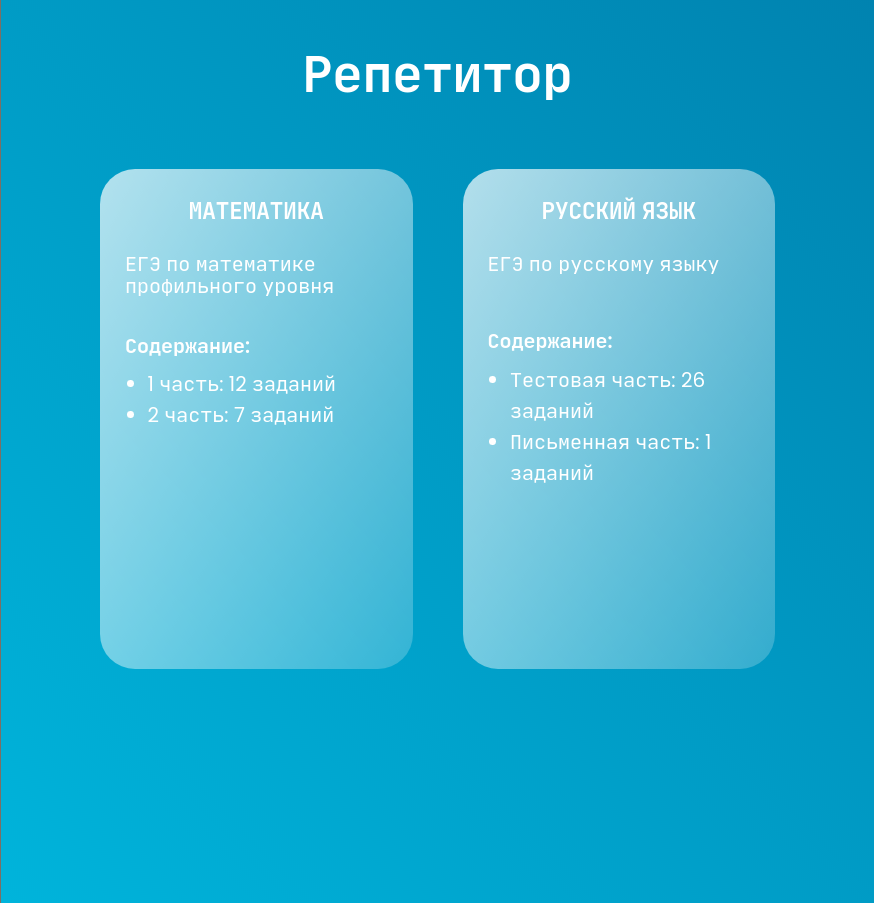
\includegraphics[height=220pt]{./img/tiles.png}
        \caption{Общий вид главной страницы}
    \end{subfigure}
    \begin{subfigure}{.5\textwidth}
        \centering
        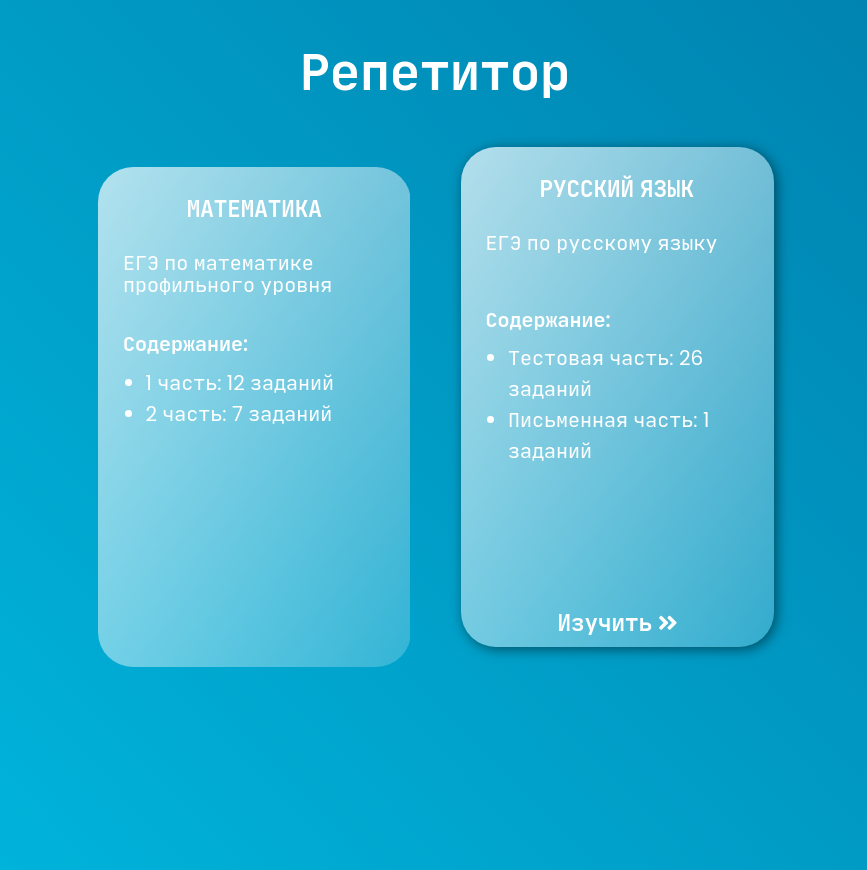
\includegraphics[height=220pt]{./img/tileHover.png}
        \caption{Активация \enquote{плитки} при наведении}
    \end{subfigure}
\end{figure}

Таким образом, получившийся интерфейс начальной страницы, на мой взгляд, не
отталкивает от себя и не дает ученику отвлечься на что-либо, не относящееся к
теме образования, напротив, он не оставляет ученику возможности перейти на
какую-нибудь стороннюю страницу, откладывая процесс подготовки. Весь выбор
посетителя состоит из двух предметов по выбору, к которым есть специальное
краткое описание.
\newpage

\subsubsection{Создание отдельных страниц для каждого предмета}
Следующим шагом в реализации моего проекта является создание страниц, на
которые посетитель попадет, кликнув по одной из табличек на начальном экране.
Для того, чтобы определиться с дизайном на данном этапе, мне предстояло сделать
выбор между строчным (представленным на Яндекс Репетиторе) и табличным
(представленным на Решу ЕГЭ) оформлением. Самой важной задачей тогда стало
размещение заданий таким образом, чтобы перейдя на страницу, приходилось делать
как можно меньше действий при выборе, однако сделать это так, чтобы ученик, не
знающий темы каждого задания, смог бы сориентироваться и выбрать нужный номер.
\\

Было принято окончательное решение создать сетку соответствующих заданий для
каждого предмета, попутно разделив их на тестовую и письменную часть как для
математики, так и для русского языка.

\begin{figure}[h]
    \begin{subfigure}{.5\textwidth}
        \centering
        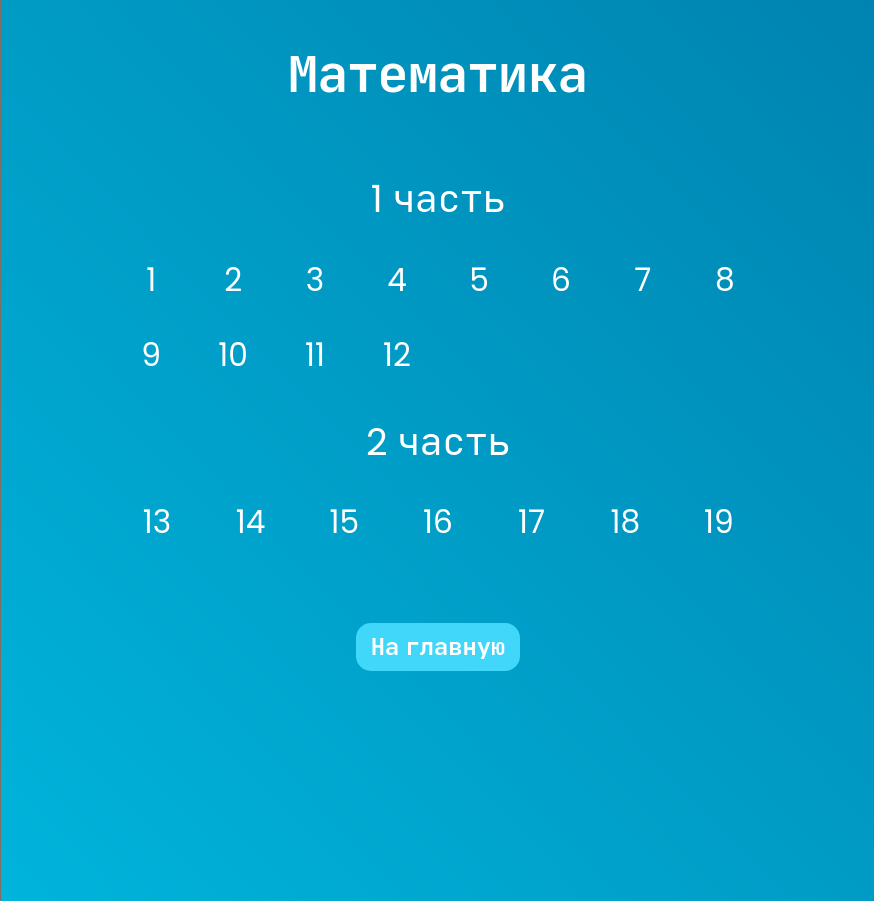
\includegraphics[height=220pt]{./img/math.png}
        \caption{Страница по математике}
    \end{subfigure}
    \begin{subfigure}{.5\textwidth}
        \centering
        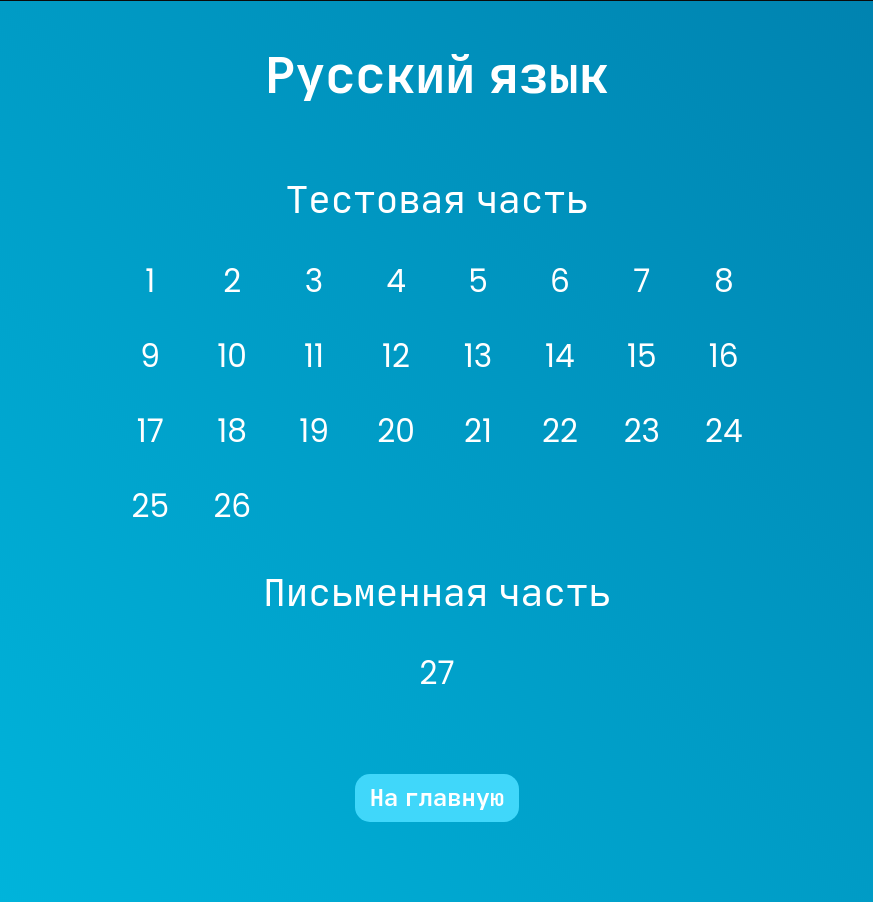
\includegraphics[height=220pt]{./img/russian.png}
        \caption{Страница по русскому языку}
    \end{subfigure}
\end{figure}

Как можно заметить, в нижней части каждой из страниц добавлена кнопка для
выхода в главное меню. Плавная анимация и неяркий фон не привлекают к кнопке
излишнего внимания и позволяют ей вписаться в общий дизайн веб-сайта.
\\

Чтобы ученик не потерялся среди номеров заданий, мною были добавлены
всплывающие подсказки под каждым из чисел, обозначающих номер задания. Эти
подсказки содержат краткую тему, по которой будут представлены задачи в каждой
из подборок, что безусловно облегчит ориентирование по сайту.

\begin{figure}[h]
    \centering
    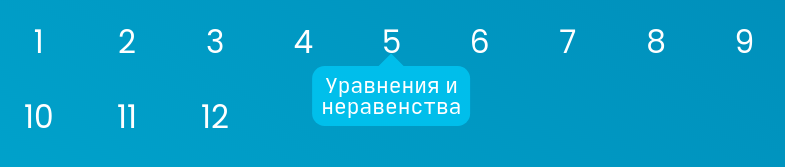
\includegraphics[height=70pt]{./img/tooltip.png}
    \caption{Всплывающая подсказка}
\end{figure}
\newpage

\subsubsection{Создание рабочей области для проведения теста}
\begin{enumerate}
    \item {\textbf{Затемнение}}\\
    Рассеивание внимания во время работы с сайтом — непосредственно то, с чем я
    борюсь, создавая свой образовательный ресурс. Затем, чтобы исключить все
    возможный отвлекающие факторы в процессе прохождения теста и тренировки, я
    создал затемнение фона при переходе в \enquote{рабочий режим}, который исключает шанс
    нажатия в ненужную область экрана.
\vspace{2mm}
\item {\textbf{\enquote{Тело} теста}}\\
    Каркасом рабочего пространства на моем сайте станет \enquote{карточка},
    озаглавленная номером задания и имеющая счетчик выполненных задач. Дизайн
    \enquote{карточки} должен также соответствовать общему дизайну сайта, что
    также включает в себя плавность появления и исчезновения карточки.
    \begin{figure}[h]
        \centering
        
\includegraphics[height=100pt]{./img/quizFrame.png}
        \caption{Общий вид рабочей области}
    \end{figure}
\item {\textbf{Содержимое теста, задачи}}\\
    Очевидно, что основным компонентом всей веб-страницы будут являться сами
    задачи и упражнения. Мне удалось собрать базу задач, представленных на
    Яндекс Репетиторе, по каждому из номеров и разместить их в отдельных
    файлах, для дальнейшей работой с ними.  Безусловно, полученное количество
    упражнения может быть увеличено путем включения в список источников задач
    других ресурсов, например, Решу ЕГЭ.
\vspace{2mm}
\item {\textbf{Размещение текста задач в каркасе}}\\
    Чтобы сделать процесс взаимодействия с сайтом как можно более приятным, а
    главное, понятным и простым данные, указанные выше, были размещены строго в
    определенных местах \enquote{тела} теста.
    \begin{figure}[h]
        \begin{subfigure}{.5\textwidth}
            \centering
            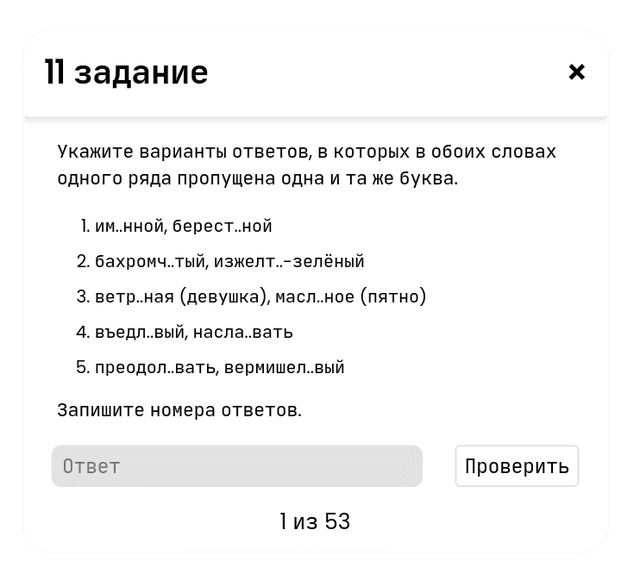
\includegraphics[height=170pt]{./img/1Example.png}
            \caption{Первый пример задачи}
        \end{subfigure}
        \begin{subfigure}{.5\textwidth}
            \centering
            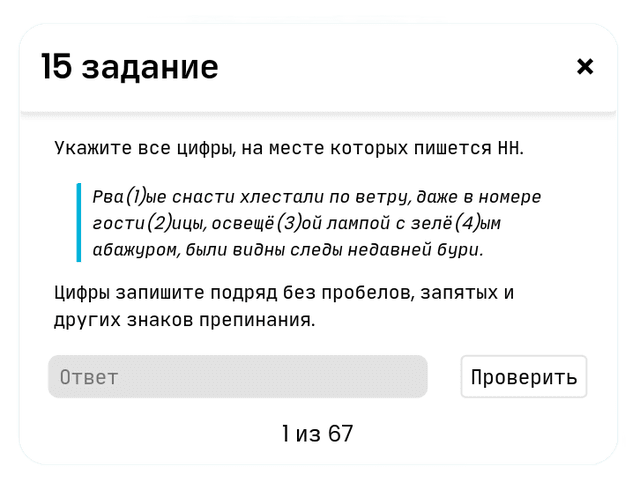
\includegraphics[height=160pt]{./img/2Example.png}
            \caption{Второй пример задачи}
        \end{subfigure}
    \end{figure}
\item {\textbf{Появление задач в случайном порядке}}\\
    При выполнении упражнений в одном и том же порядке раз за разом ученик
    станет невольно учить ответы на эту последовательность, в то время как его
    первостепенной задачей является непосредственный мыслительный процесс,
    применение полученных знаний и отработка навыков. В связи с этим
    целесообразно подбирать новую цепочку упражнений для каждого следующего
    задания.
    \begin{figure}[h]
        \begin{subfigure}{.5\textwidth}
            \centering
            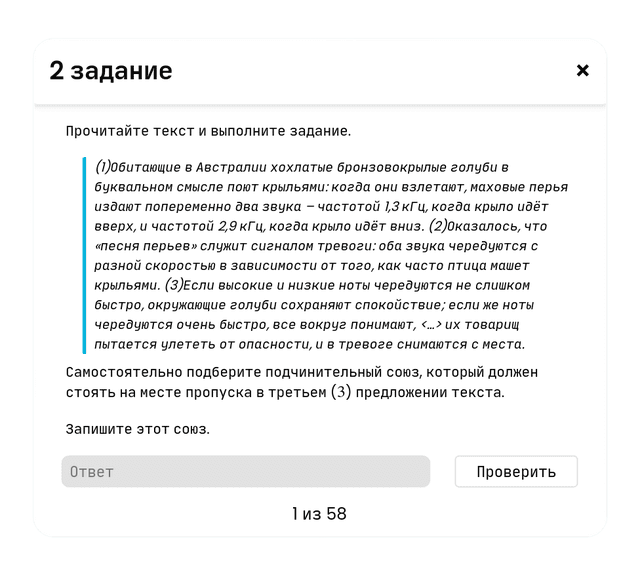
\includegraphics[height=180pt]{./img/1Sequence.png}
            \caption{Первый пример задачи}
        \end{subfigure}
        \begin{subfigure}{.5\textwidth}
            \centering
            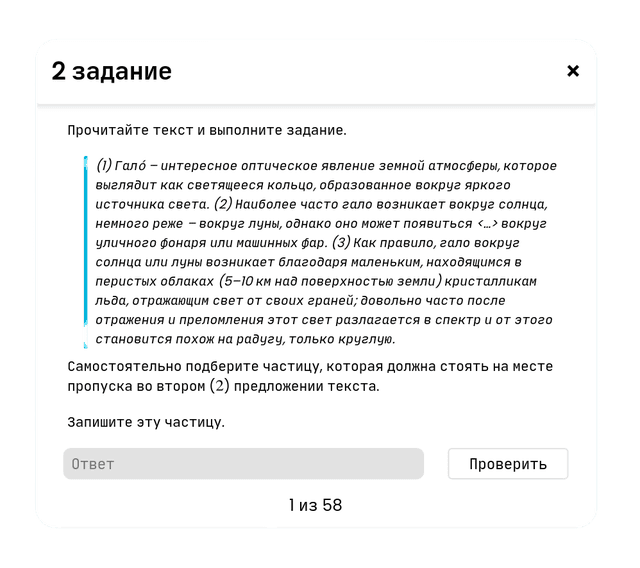
\includegraphics[height=190pt]{./img/2Sequence.png}
            \caption{Второй пример задачи}
        \end{subfigure}
    \end{figure}

\vspace{2mm}
\item {\textbf{Проверка ответа}}\\
    Для корректной работы тестирования каждый ответ, который был внесен в поле
    ввода должен быть сопоставлен с действительным ответом, а затем в
    зависимости от того, был ли он верным или нет, должен быть окрашен в
    соответствующий цвет (зеленый — правильно; красный — неправильно). В
    случае, если ответ был дан правильно, проходящий тестирование будет
    автоматически перенесен к следующей задаче.
    \begin{figure}[h]
        \begin{subfigure}{.5\textwidth}
            \centering
            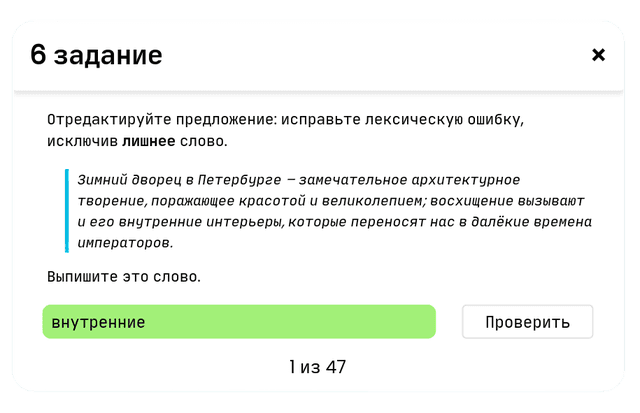
\includegraphics[height=140pt]{./img/correctAnswer.png}
            \caption{Правильный ответ}
        \end{subfigure}
        \begin{subfigure}{.5\textwidth}
            \centering
            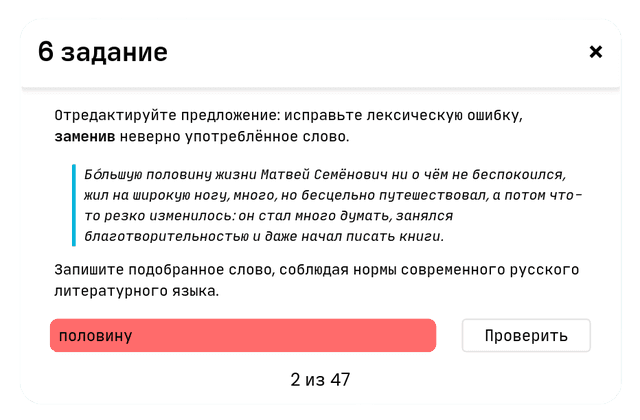
\includegraphics[height=140pt]{./img/incorrectAnswer.png}
            \caption{Неправильный ответ}
        \end{subfigure}
    \end{figure}

\end{enumerate}



\newpage

\newpage
\phantomsection
\addcontentsline{toc}{section}{Список использованных источников}
\begin{thebibliography}{9}

\bibitem{first}
Под ред. Л.Н.Боголюбова.
\textit{Готовимся к единому государственному экзамену: Обществознание.}.
М.: Дрофа, 2003.

\bibitem{second}
Под ред. В.А.Болотова.
\textit{Единый государственный экзамен. Сборник статей.}.
М.: Логос, 2002. – 208 с.
\end{thebibliography}


\end{document}
